\chapter{Preprocesado del historial de películas}

Tomaremos como ejemplo la base de datos \emph{movieslens}\footnote{\url{<http://grouplens.org/datasets/>}}, publicada en \cite{MovieLens}. Esta base de datos describe la calificación de 5 estrellas un servicio de recomendación de películas. Contiene 100836 clasificaciones en 9742 películas. Estos datos fueron creados por 610 usuarios entre el 29 de marzo de 1996 y el 24 de septiembre de 2018. Este conjunto de datos se generó el 26 de septiembre de 2018. Todos los usuarios seleccionados habían calificado al menos 20 películas. 

A continuación explicaremos los pasos realizados para la obtención del historial de usuario, y luego explicaremos como agregaremos información para que sea posible el analisis de un sistema de recomendación


\section{Descripción de la base de datos iniciales}


Los datos están contenidos en las bases de datos: 
\begin{db}[movies.csv]\label{movies}
    Esta es una base de datos donde se describe enlaza el identificador numérico de la película con el nombre y los generos a los que pertenece. A continuación se describe las variables de esta base de datos:
    
    \begin{center}
        \begin{tabular}{|c|c|c|c|c|}
        \hline
        \textbf{Variable} & \textbf{Descripción} & \textbf{Tipo} & \textbf{Ejemplo 1} & \textbf{Ejemplo 2} \\ 
        \hline
         movieId & identificador & numérico & 1 & 3431 \\  
         title & nombre  & string & 
                Toy Story (1995)  & 
                Braveheart (1995)    \\
         genres & generos  & string & Comedy|Horror & Comedy|Drama|Romance \\
         \hline
        \end{tabular}
    \end{center} 
    \hfill$\square$
\end{db}

\begin{db}[ratings.csv]\label{ratings}
    Esta es una base de datos donde se registra para cada usuario y cada película que ha visto, la puntación que ha dado. A continuación se describe las variables de esta base de datos:
    \begin{center}
        \begin{tabular}{|c|c|c|c|c|}
        \hline
        \textbf{Variable} & \textbf{Descripción} & \textbf{Tipo} & \textbf{Ejemplo 1} & \textbf{Ejemplo 2} \\ 
        \hline
         userId & identificador de usuario   & numérico & 311 & 3431 \\  
        \hline
         movieId & identificador de película & numérico & 54 & 23 \\
        \hline
         rating & puntación  & numérico & 3 & 5 \\
        \hline
        timestamp & instante de tiempo  & numérico & 964983815 & 864913515 \\        
         \hline
        \end{tabular}
    \end{center} 
    \hfill$\square$
\end{db}

\section{Union de base de datos de generos y puntaciones}
Dado que queremos ver una recuerencia en el comportamiento de los usuario es muy dificil predecir las películas de manera indivudual. Podemos preguntarnos cuantas veces el usuario va a volver a mirar la misma película. Dado que la respuesta es muy pocas, los datos de entrenamiento para la predicción de la pélicula serán muy pequeñas. Si pensamos en una película como un elemento perteneciente a un espacio vectorial de caráterísticas podemos tener más datos de entrenamiento. Por esta razón, utilizando las bases de datos (\ref{movies}) y(\ref{ratings}) creamos la base de datos (\ref{moviesref})

\begin{db}[movies\_features.csv]\label{moviesref}
Esta base de datos contiene las películas disponibles para recomendar. Cada registro de la base de datos contiene el identificador y los generos que a los que puede pertener las películas

\begin{center}
    \begin{tabular}{|c|c|c|c|c|c|c|}
    \hline
    \textbf{Variable} & \textbf{Descripción} & \textbf{Tipo} & \textbf{Ejemplo 1} & \textbf{Ejemplo 2} \\ 
    \hline
    movieId & numérico   & Identificador &    12 &  143     \\
    \hline
    title   & string     & Nombre &    "Toy Story (1995)" &  "Jumanji (1995)"     \\
    \hline
    (no genres listed)  & ¿pertenece? & boleano &  1 &  0      \\
    Action              & ¿pertenece? & boleano &  1 &  0     \\
    Adventure           & ¿pertenece? & boleano &  1 &  0      \\
    Animation           & ¿pertenece? & boleano &  1 &  0      \\
    \dots & \dots                     &  \dots &  \dots &  \dots    \\
   \hline
    \end{tabular}
\end{center}
   \hfill$\square$
\end{db}

\section{Normalización de puntación de las película}

Dado que la puntación de las películas es subjetiva, normalizaremos las puntaciones de cada usuario de manera que la peor película valorada dentro de la base de datos para cada usuario tendrá la puntación $-1$, mientras que la mejor valorada tendrá el valor de $+1$. De esta forma, evitamos la sobrevaloración o subvaloración de las películas dependiendo del usuario


\begin{db}[ratings\_norm.csv]\label{ratingsnorm}
    Esta es una base de datos (\ref{ratings}) pero donde la puntación para cada usuario esta normalizada.
    \begin{center}
        \begin{tabular}{|c|c|c|c|c|}
        \hline
        \textbf{Variable} & \textbf{Descripción} & \textbf{Tipo} & \textbf{Ejemplo 1} & \textbf{Ejemplo 2} \\ 
        \hline
         userId & identificador de usuario   & numérico & 311 & 3431 \\  
        \hline
         movieId & identificador de película & numérico & 54 & 23 \\
        \hline
         rating & puntación  & numérico & -1 & 1 \\
        \hline
        timestamp & instante de tiempo  & numérico & 964983815 & 864913515 \\        
         \hline
        \end{tabular}
    \end{center} 
    \hfill$\square$
\end{db}


\begin{obs}
    En un entorno real esta normalización no es posible debido a que no podemos saber \emph{a priori} cual será la mayor puntación que dará un usuario. En un momento dado tendremos una puntación maximan y otra minima pudiendo escalar las puntaciones. Sin embargo si en alguna iteración este máximo o minimo cambia cambiarán todas las puntaciones relativas, complicando el problema. Aunque en esta tesis no consideramos este paso, deberemos notar que en un entrono real este problema será importante.
\end{obs}


\section{Componentes principales para generos de películas}

En esta base de datos (\ref{moviesref}) tenemos 24 generos de películas. Esta forma de clasificar las películas no tiene por que se la óptima a la hora de carácterizar cada película. Con el fin de reducir la dimensionalidad de la representación de cada película, procederemos al analisis de componentes principales. Esto lo realizaremos con ayuda de la función \verb|pca()| perteneciente a la biblioteca (\cite{MATPCA}).

Nos quedaremos con las primeras componentes principales que nos den una variabilidad explicada del 90\%. En este caso en la figura (\ref{VarExp}), se puede ver que el número de componentes principales para que esta condición se cumpla es $11$.De esta manera podemos tranformar la base de datos (\ref{moviesref}) a la base de datos (\ref{movierefPCA}).

\begin{figure}[ht!]
    \centering
    \begin{subfigure}[b]{0.4\textwidth}
        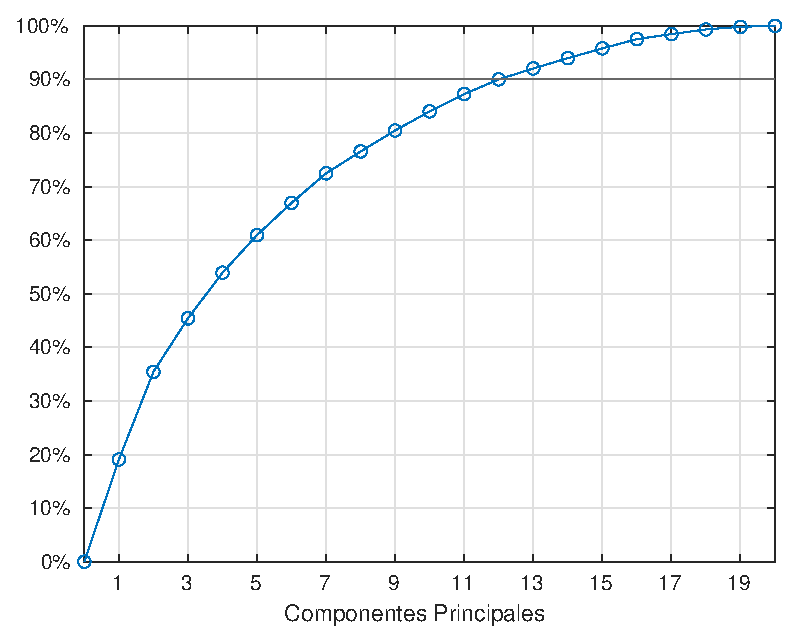
\includegraphics[scale=0.6]{img/varexp.eps}
        \caption{Variabilidad Explicada}\label{VarExp}
    \end{subfigure}
    \hspace{2cm}
    \begin{subfigure}[b]{0.4\textwidth}
        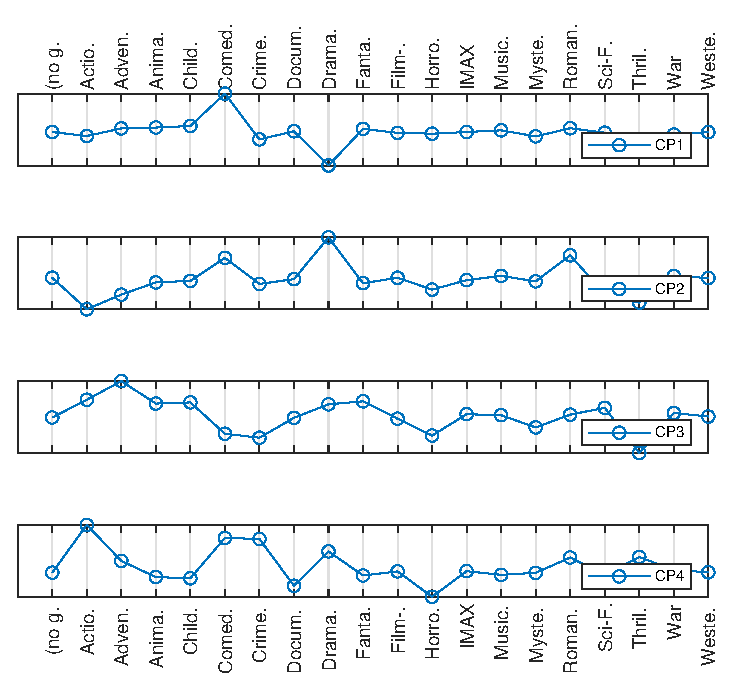
\includegraphics[scale=0.625]{img/firstPCA.eps}
        \caption{Primeras componentes}
    \end{subfigure}
    \caption{Analisis PCA en los generos de películas}
    \label{}
\end{figure}

\begin{db}[movies\_pca.csv]\label{movierefPCA}
    Esta base de datos con las componentes principales
    \begin{center}
        \begin{tabular}{|c|c|c|c|c|c|c|}
        \hline
        \textbf{Variable} & \textbf{Descripción} & \textbf{Tipo} & \textbf{Ejemplo 1} & \textbf{Ejemplo 2} \\ 
        \hline
        movieId & numérico   & Identificador &    12 &  143     \\
        \hline
        title   & string     & Nombre &    "Toy Story (1995)" &  "Jumanji (1995)"     \\
        \hline
        PC01  & Coordenada & numérico &  0.1 &  -0.3      \\
        PC02  & Coordenada & numérico &  0.5 &  0.1     \\
        PC03  & Coordenada & numérico &  1.0 &  1.0      \\
        \dots & \dots                     &  \dots &  \dots &  \dots    \\        PC11  & Coordenada & numérico &  4.0 &  -3.1      \\
       \hline
        \end{tabular}
    \end{center}
    \hfill $\square$
\end{db}


\section{Historial de aceptación para cada usuario}


Para ello, cruzaremos la base de datos \emph{movies.csv} y \emph{rating.csv}, para crear una nueva base de datos que en sus variables contenga cada uno de los generos disponibles en la totalidad de los datos. 

\begin{db}[user\_movies\_accept.csv]\label{user_movies_features}
    Esta es una base de datos que registra las interacciones de distintos usuarios con las distintas películas, además de informar del vector de caráterísticas de cada película vista.
    \begin{center}
        \begin{tabular}{|c|c|c|c|c|}
        \hline
        \textbf{Variable} & \textbf{Descripción} & \textbf{Tipo} & \textbf{Ejemplo 1} & \textbf{Ejemplo 2} \\ 
        \hline
            userId & identificador de usuario   & numérico & 311 & 3431 \\  
        \hline
            rating & puntación  & numérico & 3 & 5 \\
        \hline
        timestamp & instante de tiempo  & numérico & 964983815 & 864913515 \\        
        \hline
        PC01  & Coordenada & numérico &  0.1 &  -0.3      \\
        PC02  & Coordenada & numérico &  0.5 &  0.1     \\
        PC03  & Coordenada & numérico &  1.0 &  1.0      \\
        \dots & \dots                     &  \dots &  \dots &  \dots    \\        PC11  & Coordenada & numérico &  4.0 &  -3.1      \\
            \hline
        \end{tabular}
    \end{center}
    \hfill$\square$         
\end{db}



Si consideramos que tenemos $d$ géneros, entonces para cada usuario tenemos una secuencia de vectores $\bm{x}_t \in [0,1]^d \ | \ \forall t \in \{ 1,\dots,T\}$. Por último, si una película pertenece a varios géneros a la vez, el módulo del vector asociado será más grande que una película con menos géneros asociados. Dado que el módulo de un vector puede afectar a los modelos de prodicción normalizaremos todos los vectores $\bm{x}_d$. 

Asi pues, el historial de un usuario se puede entender como la rotación de un vector $\bm{x}_t$:

\begin{gather}
    \{ \bm{x}_t  \}_{t \geq0} \in \mathbb{R}^d \ \ | \ ||\bm{x}_t|| = 1 \ \forall t \leq 0
\end{gather}



\section{Generación sintética del historial de rechazo}

El problema que tenemos en estos datos es que solo tenemos las películas que el usuario ha seleccionado en cada iteración, sin embago si consideramos el proceso de recomendación en cada iteración el usuario se le ha recomendado una serie de peliculas de las cuales solo tenemos constancia la película que ha seleccionado. Es por ello que consideraremos que en cada iteración el sistema de recomendación a ofrecido dos películas al usuario. Una de ella la ha aceptado y la otra la ha rechazado. Para crear el historial de películas rechazadas agregaremos de manera ficticia otra película que tengamos en el historial del usuario pero que tenga menor puntación que la película que ha selecionado en la realidad. 

\begin{db}[user\_movies\_reject.csv]\label{user_movies_features_reject}
    Base de datos con la misma estructura y la mismas instancias que la base de datos (\ref{user_movies_features}), pero esta contiene las películas que el usuario ha rechazado.
    \begin{center}
        \begin{tabular}{|c|c|c|c|c|}
        \hline
        \textbf{Variable} & \textbf{Descripción} & \textbf{Tipo} & \textbf{Ejemplo 1} & \textbf{Ejemplo 2} \\ 
        \hline
            userId & identificador de usuario   & numérico & 311 & 3431 \\  
        \hline
            \st{rating} & -  & - & - & - \\
        \hline
        timestamp & instante de tiempo  & numérico & 964983815 & 864913515 \\        
        \hline
        PC01  & Coordenada & numérico &  0.1 &  -0.3      \\
        PC02  & Coordenada & numérico &  0.5 &  0.1     \\
        PC03  & Coordenada & numérico &  1.0 &  1.0      \\
        \dots & \dots                     &  \dots &  \dots &  \dots    \\        PC11  & Coordenada & numérico &  4.0 &  -3.1      \\
            \hline
        \end{tabular}
    \end{center}
    \hfill $\square$
\end{db}
\begin{obs}
    Para el historial de aceptación tambien tenemos su correspondiente puntación, sin embargo para el historial de rechazos dado que el usuario no lo ha selecionado, en general no tenemos puntación asociada.
\end{obs}


    


\section{Bases de datos finales: Historiales de usuarios}\label{HObt}


En la figura (\ref{DFPrePro}) mostramos un diagrama de flujo de como hemos creado los historiales de usuario que finalmente se utilizarán para entrenar un proceso de deción de Markov. 

Finalmente para cada usuario tenemos: el historial de películas aceptadas y el historial de rechazadas.
\begin{itemize}
    \item Tenemos la acciones en cada iteración: 
    \begin{gather}
        \{\bm{a}_t\}_{t\geq 0} =\{ \bm{x}_t^a,\bm{x}_t^r\}_{t\geq 0}
    \end{gather}

    \item Tenemos el estado en cada iteración: 
    \begin{gather}
        \{\bm{s}_t\}_{t\geq 0} = \{ \bm{x}_t^a\}_{t \geq 0}
    \end{gather}

    
\end{itemize}

Denotaremos al historial de un usuario como 
\begin{gather}
    \mathcal{H} = \{ \bm{x}_t^r,\bm{x}_t^a\}_{t \geq 0}
\end{gather}
 
Mostramos como ejemplo la siguiente tabla como historial de aceptación (base de datos \ref{user_movies_features}):
\begin{center}
    \begin{tabular}{|c|c|c|c|c|c|c|}
\hline
\textbf{title}          &              \textbf{rating}  &  \textbf{timestamp}   &    \textbf{Action}   &  \textbf{Adventure} & \dots \\
\hline
"The Drop (2014)"                   &      2   &   1.4795e+09  &       0        & 0  & \dots \\  
"Django Unchained (2012)"           &    3.5   &   1.4795e+09  &       0.57735  & 0  & \dots \\ 
"Interstellar (2014)"               &      3   &   1.4795e+09  &       0        & 0  & \dots \\  
"The Drop (2014)"                   &      2   &   1.4795e+09  &       0        & 0  & \dots \\  
"The Drop (2014)"                   &      2   &   1.4795e+09  &       0        & 0  & \dots \\  
"Exit Through the Gift Shop (2010)" &      3   &   1.4795e+09  &       0        & 0  & \dots \\  
"Collateral (2004)"                 &    3.5   &   1.4795e+09  &       0.5      & 0  & \dots \\  
    \hline
    \end{tabular}
\end{center}

Además del historial de rechazo (base de datos \ref{user_movies_features_reject}):

\begin{center}
    \begin{tabular}{|c|c|c|c|c|c|c|}
\hline
\textbf{title}          &              \textbf{rating}  &  \textbf{timestamp}   &    \textbf{Action}   &  \textbf{Adventure} & \dots \\
\hline
"The Drop (2014)"                   &      2   &   1.4795e+09  &       0        & 0  & \dots \\  
"Django Unchained (2012)"           &    3.5   &   1.4795e+09  &       0.57735  & 0  & \dots \\ 
"Interstellar (2014)"               &      3   &   1.4795e+09  &       0        & 0  & \dots \\  
"The Drop (2014)"                   &      2   &   1.4795e+09  &       0        & 0  & \dots \\  
"The Drop (2014)"                   &      2   &   1.4795e+09  &       0        & 0  & \dots \\  
"Exit Through the Gift Shop (2010)" &      3   &   1.4795e+09  &       0        & 0  & \dots \\  
"Collateral (2004)"                 &    3.5   &   1.4795e+09  &       0.5      & 0  & \dots \\  
    \hline
    \end{tabular}
\end{center}



\tikzstyle{startstop} = [rectangle, rounded corners, minimum width=1.5cm, minimum height=1.cm,text centered, draw=black, fill=blue!30,line width=1.25pt]
%
\tikzstyle{cir} = [circle, rounded corners, minimum width=1.05cm, minimum height=0.5cm,text centered, draw=black, fill=green!30,line width=1.25pt]
%
\tikzstyle{cir_hd} = [circle, rounded corners, minimum width=0.5cm, minimum height=0.5cm,text centered, draw=black, fill=red!30,line width=1.25pt]
%%%%%%%%%%%%%%%%%%%%%%%%%%%%%%%%%%%%%%%%%%%%%%%
% for double arrows a la chef
% adapt line thickness and line width, if needed
\tikzstyle{vecArrow} = [thick, decoration={markings,mark=at position
   1 with {\arrow[semithick]{open triangle 60}}},
   double distance=1.4pt, shorten >= 5.5pt,
   preaction = {decorate},
   postaction = {draw,line width=2.4pt, white,shorten >= 4.5pt}]
\tikzstyle{innerWhite} = [semithick, white,line width=1.4pt, shorten >= 4.5pt]

\begin{figure}[]
    \centering
        
\begin{tikzpicture}[node distance=2.05cm] 
    \filldraw[color=red!60, fill=red!5, very thick](-1.7,1.4) rectangle (1.55,-2.7);
    \filldraw[color=blue!60, fill=blue!5, very thick](1.65,1.4) rectangle (8.2,-2.7);
    \filldraw[color=green!60, fill=green!5, very thick](8.30,1.4) rectangle (12.70,-2.7);

    \node[draw,fill=red!20] at   (-0.1,1.0) {\small \textbf{B.D. de Entrada}};
    \node[draw,fill=blue!20] at  (4.9   ,1.0) {\small \textbf{B.D. Intermedias}};
    \node[draw,fill=green!20] at (10.5   ,1.0) {\small \textbf{B.D de Salida}};



    \node (movies) [startstop] {\small movies.csv};
    \node (ratings) [startstop,below of=movies] {\small ratings.csv};

    \node (ratingsnorm) [startstop,right of=ratings,xshift=3cm] {\small ratings\_norm.csv};

    \node (moviesfeatures) [startstop, right of=movies,xshift=1.5cm] {\small movies\_features.csv};

    \node (moviespca) [startstop, right of=moviesfeatures,xshift=1cm] {\small movies\_pca.csv};

    \node (usermovies) [startstop,  right of=ratings,xshift=8.5cm] {\small user\_movies\_accept.csv};
    %
    \node (usermoviesreject) [startstop,above of=usermovies] {\small user\_movies\_reject.csv};
%%%%%
    \draw  [line width=1.25pt,bend left=0,<-] (moviesfeatures) edge (movies);
    \draw  [line width=1.25pt,bend left=0,<-] (moviespca) edge (moviesfeatures);
    \draw  [line width=1.25pt,bend left=10,<-] (usermovies) edge (moviespca);

    \draw  [line width=1.25pt,bend left=0,<-] (ratingsnorm) edge (ratings);
    \draw  [line width=1.25pt,bend left=0,<-] (usermovies) edge (ratingsnorm);

    \draw  [line width=1.25pt,bend left=0,<-] (usermoviesreject) edge (usermovies);

\end{tikzpicture}

    \caption{Diagrama de flujo para el preprocesado de los datos.}{En rojo las base de datos obtenidas de \cite{MovieLens}, en azul las bases de datos creadas como pasos Intermedias y finalmente en verde las bases de datos que se usarán en esta tesis.}
    \label{DFPrePro}


\end{figure}
